\chapter{Wheels and satellites}
\label{ch:wheels}

Chapter~\ref{ch:vio} ended with two weaknesses of visual--inertial
odometry. It drifts along four directions that nothing in it can see:
position and heading. And on a straight row, its accelerometer bias is
tied to its tilt, so a blind spell before the first turn is expensive.
A mower carries two more sensors that address exactly these. Its
\emph{wheels} measure its speed, and its motion is constrained: it rolls
forward, it does not slide sideways. A \emph{GNSS receiver} with RTK
corrections measures the position of its antenna to a centimetre or
two, in a frame attached to the Earth, under open sky. This chapter
turns both into factors of the VIO window, shows how to bring the VIO's
arbitrary frame into the Earth's, and studies what happens under the
trees, where the satellites become unreliable.

\section{Wheels}

\begin{definition}{Differential drive}{diffdrive}
A vehicle with two independently driven wheels on a common axle, of
track width $b$, whose wheels roll without slipping with speeds $v_l$
and $v_r$, moves its axle centre forward with speed $v$ and turns with
yaw rate $\omega$:
\begin{equation}\label{eq:diffdrive}
v=\tfrac12(v_l+v_r),\qquad\omega=\frac{v_r-v_l}{b}.
\end{equation}
\end{definition}

Ride-on mowers with two hydrostatic drives and zero-turn mowers are
differential drives. A mower with a steered front axle follows the
bicycle model instead, but the same two quantities, forward speed and
yaw rate, come out of it.

\begin{proposition}{Planar dead reckoning}{deadreck}
Integrate the planar pose $(x,y,\psi)$ over steps of $\Delta t$ with the
midpoint heading $\bar\psi=\psi+\frac12\omega\Delta t$:
$x\leftarrow x+v\Delta t\cos\bar\psi$, $y\leftarrow y+v\Delta t\sin\bar\psi$,
$\psi\leftarrow\psi+\omega\Delta t$. If $v$ and $\omega$ carry independent
white errors of densities $\sigma_v$ and $\sigma_\omega$, the pose
covariance propagates to first order as $P\leftarrow FPF\T+GQG\T$ with
$Q=\diag(\sigma_v^2,\sigma_\omega^2)/\Delta t$ and
\begin{equation}\label{eq:odocov}
F=\begin{pmatrix}1&0&-v\Delta t\sin\bar\psi\\0&1&v\Delta t\cos\bar\psi\\
0&0&1\end{pmatrix},\qquad
G=\begin{pmatrix}\Delta t\cos\bar\psi&-\frac12v\Delta t^2\sin\bar\psi\\
\Delta t\sin\bar\psi&\frac12v\Delta t^2\cos\bar\psi\\0&\Delta t
\end{pmatrix}.
\end{equation}
\end{proposition}

\begin{proof}
$F$ and $G$ are the Jacobians of the update with respect to the pose and
to $(v,\omega)$. The heading enters through $\bar\psi$, with
$\partial\bar\psi/\partial\psi=1$ and $\partial\bar\psi/\partial\omega=
\frac12\Delta t$. The per-sample covariance of the inputs comes from
\cref{prop:discnoise}. The errors of successive steps are independent of
the current pose error, so the covariances add.
\end{proof}

White errors are the harmless part. The harmful ones are systematic.
Let the effective radii of the two wheels be wrong by fractions
$\epsilon_l$ and $\epsilon_r$. The measured yaw rate is then off by
$v(\epsilon_r-\epsilon_l)/b$, and after a distance $D$ the heading is
off by
\begin{equation}\label{eq:wheelyaw}
\delta\psi\approx\frac{(\epsilon_r-\epsilon_l)\,D}{b}.
\end{equation}
For our simulated mower, $\epsilon_l=1\,\%$, $\epsilon_r=-0.8\,\%$ and
$b=1$\,m, so over the 65\,m of the drive $\delta\psi=1.17$\,rad, or
$67^\circ$. The simulation gives $68^\circ$ and an error of 8.9\,m at
the end (\cref{fig:wheels}, left). Grass makes it worse: in tight turns
on wet grass the wheels \emph{slip} (they turn faster than the mower
moves), and on a slope they slide sideways.

The fix is to take the heading from the gyroscope and only the speed
from the wheels. A gyroscope bias of $0.01^\circ$/s, known from the
still phase, costs less than a degree over the drive, and the final
error falls to 0.37\,m. In the VIO, the gyroscope is already there; what
the wheels add is the velocity.

\begin{proposition}{The wheel factor}{wheelfactor}
Let the body origin be at the axle centre, and let the wheels measure
the forward speed $s$. The \emph{wheel factor} of a keyframe state is
\begin{equation}\label{eq:wheelres}
\vect{r}=\Sigma_w^{-1/2}\bigl(R\T\vect{v}-(s,0,0)\T\bigr),\qquad
\Sigma_w=\diag(\sigma_s^2,\sigma_{\mathrm{lat}}^2,\sigma_{\mathrm{vert}}^2).
\end{equation}
Its second and third rows are the \emph{non-holonomic constraint}: the
axle does not move sideways or vertically in the body frame. Its
Jacobians are
\[
\frac{\partial\vect{r}}{\partial\delta\bphi}=\Sigma_w^{-1/2}\hatop{(R\T
\vect{v})},\qquad
\frac{\partial\vect{r}}{\partial\delta\vect{v}}=\Sigma_w^{-1/2}R\T,
\]
and zero for the position and the biases.
\end{proposition}

\begin{proof}
$(R\Exp(\delta\bphi))\T\vect{v}=\Exp(-\delta\bphi)R\T\vect{v}\approx R\T
\vect{v}-\hatop{\delta\bphi}R\T\vect{v}=R\T\vect{v}+\hatop{(R\T\vect{v})}
\delta\bphi$. The velocity enters linearly.
\end{proof}

The standard deviations are not those of the encoders. They must cover
what the factor does not model: the bumps, which give the axle a
vertical velocity of a few cm/s; the scale error of the wheels; and
slip. Our implementation uses $\sigma_s=2$\,cm/s and
$\sigma_{\mathrm{lat}}=\sigma_{\mathrm{vert}}=5$\,cm/s with a Huber kernel.
The factor is evaluated at the keyframes, from the encoder sample
nearest in time; an implementation on a real machine would preintegrate
the wheel speeds between keyframes, as the IMU's are.

\begin{figure}[ht]
\centering
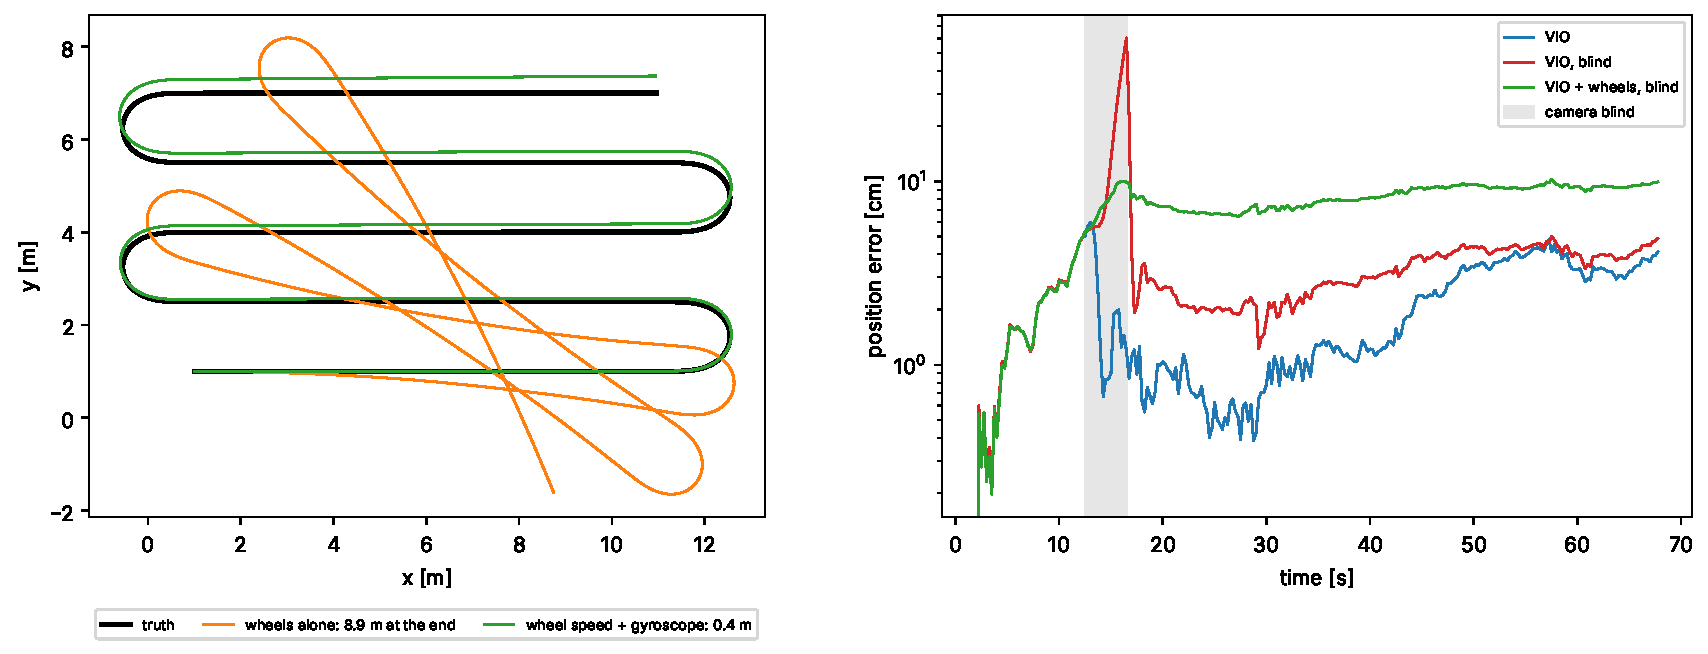
\includegraphics[width=\linewidth]{figures/ch14_wheels.pdf}
\caption{Left: dead reckoning with the wheels alone (a 1.8\,\% radius
mismatch between the wheels) and with the wheel speed and the
gyroscope's heading. Right: the VIO with the camera blind for 4\,s in
the first turn (\cref{fig:viotraj}), without and with the wheel factor.}
\label{fig:wheels}
\end{figure}

With the camera blind for 4\,s in the first turn, the VIO of
Chapter~\ref{ch:vio} drifted to 60\,cm on its unresolved accelerometer
bias. With the wheel factor the velocity cannot drift, and the error
peaks at about 10\,cm (\cref{fig:wheels}, right). There is a price,
though. With the camera working, the wheel factor makes the VIO slightly
\emph{worse}: 3.0\,cm RMS instead of 2.5\,cm. The wheels' scale error
(1\,\%) and their slip in the turns are biases, not noise, and the
factor passes them on. The remedy is to estimate what is systematic:
the wheel radii, or a single scale factor, as additional states, which
the vision makes observable while it works. That is the approach of the
``VINS on wheels'' line of work. A cheaper remedy is to switch the
factor on only when the vision is weak.

\section{RTK-GNSS}

A GNSS receiver measures its distance to each satellite in view from
the travel time of the signal (the \emph{code}, metres of accuracy) and
from the phase of the carrier (millimetres, but up to an unknown whole
number of wavelengths of about 19\,cm). Real-time kinematic positioning
(RTK) uses a \emph{base station} at a known position, nearby or through
an NTRIP correction service. Most errors (satellite clocks and orbits,
the ionosphere and troposphere) are the same at the base and at the
rover, and differencing the two receivers' measurements cancels them.
Once the integer numbers of wavelengths are resolved, the solution is
\emph{fixed} and its error is about a centimetre horizontally and twice
that vertically. If they cannot be resolved, the solution is
\emph{float}, with errors of decimetres that wander slowly.

Two things break RTK in a garden. Trees attenuate and scatter the
signals, so the receiver tracks fewer satellites and loses the fix under
a canopy. Walls and roofs reflect the signals (\emph{multipath}), so a
reflected path, longer than the direct one, can produce a position off
by metres while the receiver still reports a small uncertainty. The
simulated receiver in \code{fusion.RTKReceiver} reproduces both. Under
the canopy of the young tree in the lawn (2.5\,m around its trunk) and
near the house, it delivers float solutions, a wandering error of about
25\,cm that it under-reports as 10\,cm, and multipath outliers of 1 to
3\,m on 15\,\% of the epochs. Elsewhere it delivers fixes with 1.5\,cm
of error.

\subsection*{Coordinates}

A receiver reports latitude, longitude and height on the WGS84
ellipsoid. The mower needs metres in a local frame. The natural choice
is an east--north--up (ENU) frame at a reference point near the garden:
its $z$ axis is the local vertical, which is the direction of gravity
up to the deflection of the vertical (a few arcseconds), so it can be
identified with the world frame of the VIO.

\begin{proposition}{Geodetic, ECEF and ENU coordinates}{enu}
A point of latitude $\varphi$, longitude $\lambda$ and ellipsoidal height
$h$ has Earth-centred, Earth-fixed (ECEF) coordinates
\begin{equation}\label{eq:ecef}
\vect{x}=\begin{pmatrix}(N+h)\cos\varphi\cos\lambda\\(N+h)\cos\varphi
\sin\lambda\\\bigl(N(1-e^2)+h\bigr)\sin\varphi\end{pmatrix},\qquad
N=\frac{a}{\sqrt{1-e^2\sin^2\varphi}},
\end{equation}
with $a$ and $e^2$ the semi-major axis and squared eccentricity of the
ellipsoid. At a reference point $(\varphi_0,\lambda_0)$ with ECEF
position $\vect{x}_0$, the ENU coordinates are $R_{\mathrm{enu}}(\vect{x}-
\vect{x}_0)$, where the rows of $R_{\mathrm{enu}}$ are
\begin{equation}\label{eq:renu}
\vect{e}=\begin{pmatrix}-\sin\lambda_0\\\cos\lambda_0\\0\end{pmatrix},\quad
\vect{n}=\begin{pmatrix}-\sin\varphi_0\cos\lambda_0\\-\sin\varphi_0
\sin\lambda_0\\\cos\varphi_0\end{pmatrix},\quad
\vect{u}=\begin{pmatrix}\cos\varphi_0\cos\lambda_0\\\cos\varphi_0
\sin\lambda_0\\\sin\varphi_0\end{pmatrix}.
\end{equation}
\end{proposition}

\begin{proof}
In the meridian plane of the point, with coordinates $\rho$ (distance from
the axis) and $z$, the ellipsoid is the ellipse $\rho=a\cos\beta$,
$z=b\sin\beta$, $b=a\sqrt{1-e^2}$. Its tangent is $(-a\sin\beta,b\cos
\beta)$, so its outward normal is along $(b\cos\beta,a\sin\beta)$. The
geodetic latitude is the angle of that normal: $\tan\varphi=\frac ab
\tan\beta$, i.e.\ $\tan\beta=\sqrt{1-e^2}\tan\varphi$. Then
\[
\cos\beta=\frac1{\sqrt{1+(1-e^2)\tan^2\varphi}}=\frac{\cos\varphi}{\sqrt{1-
e^2\sin^2\varphi}},
\]
so $\rho=a\cos\beta=N\cos\varphi$ and
$z=b\sin\beta=b\tan\beta\cos\beta=a(1-e^2)\sin\varphi/\sqrt{1-e^2\sin^2
\varphi}=N(1-e^2)\sin\varphi$. Moving a distance $h$ along the unit normal
$(\cos\varphi,\sin\varphi)$ adds $h\cos\varphi$ to $\rho$ and $h\sin\varphi$
to $z$, and rotating the meridian plane by $\lambda$ about the $z$ axis
gives \eqref{eq:ecef}. The vector $\vect{u}$ is that unit normal at the
reference point; $\vect{e}$ is $\partial\vect{x}/\partial\lambda$
normalised, the direction of increasing longitude; and $\vect{n}=\vect{u}
\times\vect{e}$ completes a right-handed orthonormal basis.
\end{proof}

The inverse, from ECEF to latitude and height, has no simple closed
form. The function \code{fusion.ecef\_to\_geodetic} iterates on the
latitude, and converges to well below a millimetre in a few steps. Over a
garden, the curvature of the Earth is negligible: the ENU plane departs
from the ellipsoid by about $d^2/(2a)$, $8\,\mu$m at 10\,m.

\subsection*{The GNSS factor}

The antenna is not at the body origin. On a mower it sits on a mast,
here 1.4\,m above the ground and 0.4\,m behind the axle, so its position
is $\p+R\,\vect{t}_{\mathrm{ant}}$.

\begin{proposition}{The GNSS factor}{gnssfactor}
An RTK position $\z$ (ENU) with covariance $\Sigma_z$ gives the factor
\begin{equation}\label{eq:gnssres}
\vect{r}=\Sigma_z^{-1/2}\bigl(\p+R\,\vect{t}_{\mathrm{ant}}-\z\bigr),
\qquad
\frac{\partial\vect{r}}{\partial\delta\bphi}=-\Sigma_z^{-1/2}R\,\hatop{
\vect{t}_{\mathrm{ant}}},\qquad
\frac{\partial\vect{r}}{\partial\delta\p}=\Sigma_z^{-1/2}R,
\end{equation}
with zero Jacobians for the velocity and the biases.
\end{proposition}

\begin{proof}
$\p+R\delta\p+R\Exp(\delta\bphi)\vect{t}_{\mathrm{ant}}\approx\p+R
\vect{t}_{\mathrm{ant}}+R\delta\p+R\hatop{\delta\bphi}\vect{t}_{\mathrm{ant}}$,
and $\hatop{\delta\bphi}\vect{t}=-\hatop{\vect{t}}\delta\bphi$.
\end{proof}

The GNSS factor removes the unobservable directions of
\cref{thm:vionull}: positions are measured directly, and as soon as two
measured positions are at different places, the direction between them
fixes the heading. It also anchors the map of Chapter~\ref{ch:maps} to the
Earth, so that a lawn boundary surveyed once stays valid from one
session to the next.

The lever arm matters. Its horizontal part rotates with the heading,
by $0.8$\,m between the two directions of a row, and its vertical part
turns every tilt of the mower into a horizontal displacement of the
antenna, $1.4$\,m$\times1^\circ=2.4$\,cm. Leaving it out costs up to
24\,cm in the turns (\cref{fig:gnss}).

GNSS also provides time. A receiver delivers a pulse per second aligned
to GPS time to within tens of nanoseconds, which is how the camera and
the IMU of Chapter~\ref{ch:vio} can be timestamped on a common clock.

\section{From the VIO frame to the Earth}

The VIO starts in a frame of its own: its $z$ axis is vertical (gravity
fixes it), but its heading and origin are arbitrary. Before GNSS factors
can enter the window, the window must be expressed in ENU. By
\cref{thm:vionull}, the transformation needed is a rotation about the
vertical and a translation, four degrees of freedom. Moving the whole
window by such a transformation leaves its cost unchanged, prior
included (\code{SlidingWindowVIO.transform}; the test suite checks it).

\begin{proposition}{4-DoF alignment}{align4}
Let $\vect{a}_i$ be points in one frame and $\vect{b}_i$ the same points
in another, $i=1,\dots,n$, with centroids $\bar{\vect{a}}$ and
$\bar{\vect{b}}$ and centred coordinates $\vect{a}_i'$ and $\vect{b}_i'$.
The rotation $R_z(\psi)$ about the vertical and the translation
$\vect{t}$ minimising $\sum_i\norm{\vect{b}_i-R_z(\psi)\vect{a}_i-
\vect{t}}^2$ are
\begin{equation}\label{eq:align4}
\psi=\operatorname{atan2}\Bigl(\sum_i(a'_{ix}b'_{iy}-a'_{iy}b'_{ix}),\;
\sum_i(a'_{ix}b'_{ix}+a'_{iy}b'_{iy})\Bigr),\qquad
\vect{t}=\bar{\vect{b}}-R_z(\psi)\bar{\vect{a}}.
\end{equation}
\end{proposition}

\begin{proof}
For fixed $\psi$ the cost is quadratic in $\vect{t}$ and minimised at
$\vect{t}=\bar{\vect{b}}-R_z\bar{\vect{a}}$, which leaves
$\sum_i\norm{\vect{b}_i'-R_z\vect{a}_i'}^2$. The vertical components do
not depend on $\psi$. Horizontally, $\norm{\vect{b}'-R_z\vect{a}'}^2=
\norm{\vect{a}'}^2+\norm{\vect{b}'}^2-2\vect{b}'\cdot R_z\vect{a}'$ and
$\vect{b}'\cdot R_z\vect{a}'=\cos\psi\,(a'_xb'_x+a'_yb'_y)+\sin\psi\,
(a'_xb'_y-a'_yb'_x)$. Writing the two sums as $C$ and $S$, we must
maximise $C\cos\psi+S\sin\psi=\sqrt{C^2+S^2}\cos(\psi-\operatorname{atan2}
(S,C))$, which gives \eqref{eq:align4}. (This is \cref{prop:umeyama}
restricted to rotations about one axis.)
\end{proof}

How accurately is the heading determined? While the mower drives a
straight line, the alignment amounts to fitting the direction of that
line through the GNSS fixes.

\begin{proposition}{Heading from a straight drive}{headingline}
Let $n$ fixes be spread evenly along a straight segment of length $L$,
each with independent error of standard deviation $\sigma$ across the
segment, and let the positions along the segment be exact. To first
order, the heading of the least-squares line through them has standard
deviation
\begin{equation}\label{eq:headingline}
\sigma_\psi\approx\frac{\sigma\sqrt{12}}{L\sqrt n}.
\end{equation}
\end{proposition}

\begin{proof}
In coordinates along ($s$) and across ($c$) the segment, the fit is a
straight-line regression $c=\alpha+\beta s$, whose slope estimate has
variance $\sigma^2/\sum_i(s_i-\bar s)^2$. For $n$ evenly spaced points on
a segment of length $L$, $\sum_i(s_i-\bar s)^2\approx nL^2/12$ (the
variance of the uniform distribution on $[0,L]$ is $L^2/12$). For small
angles, $\psi\approx\beta$.
\end{proof}

\begin{figure}[ht]
\centering
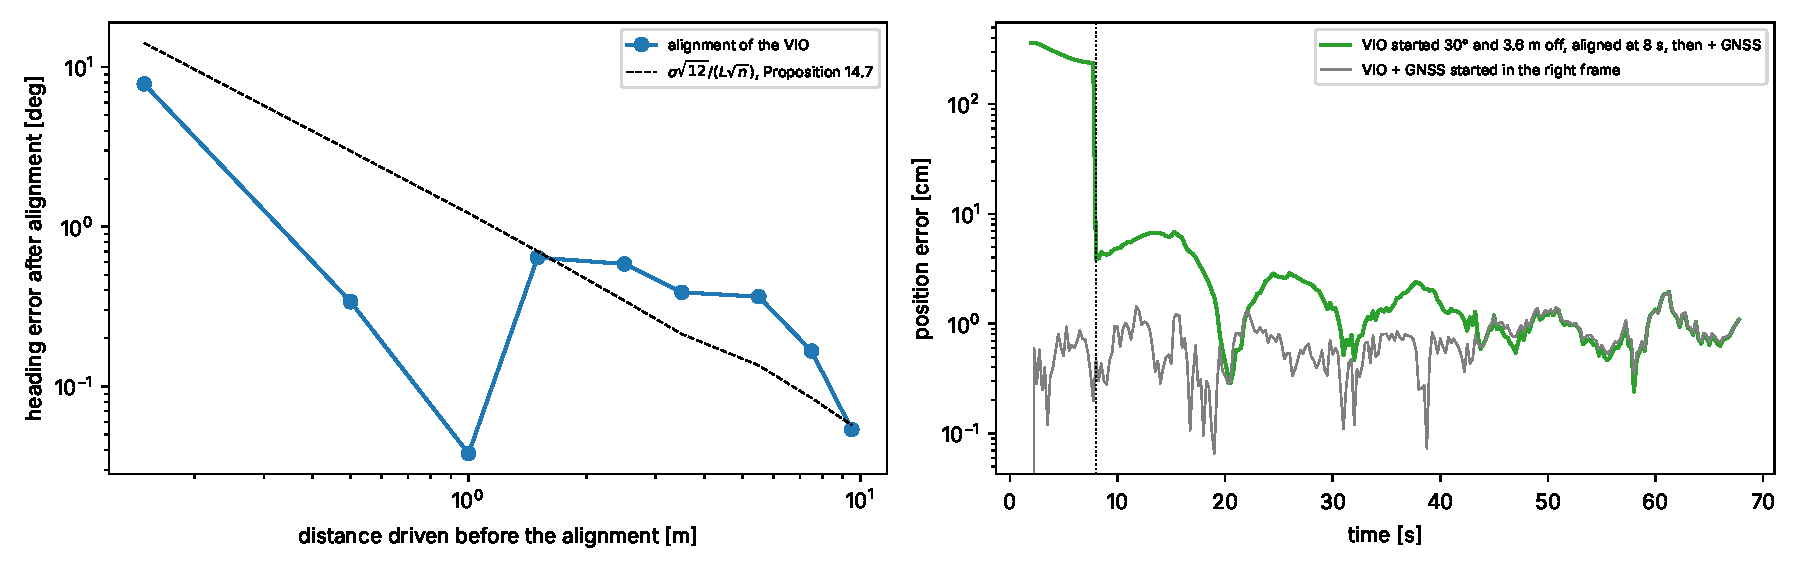
\includegraphics[width=\linewidth]{figures/ch14_align.pdf}
\caption{Left: heading error of the 4-DoF alignment of a VIO started
$30^\circ$ off, against the distance driven before aligning, and the
first-order prediction \eqref{eq:headingline}. Right: that VIO, aligned
after 8\,s and then fused with the GNSS factors, against one started in
the right frame.}
\label{fig:align}
\end{figure}

With fixes at 4\,Hz, 1.5\,cm of noise and 1\,m/s, a 10\,m drive
determines the heading to $0.05^\circ$ (\cref{fig:align}, left: the
measured errors scatter around the prediction). In the full experiment,
the VIO starts $30^\circ$ and 3.6\,m off. It is aligned after 8\,s on
the 16 fixes taken before the tree's canopy, which corrects
$30.35^\circ$ of heading. From then on, the GNSS factors make it
indistinguishable from a VIO started in the right frame, and it ends
with an error of 1.1\,cm.

\section{Results}

\begin{figure}[ht]
\centering
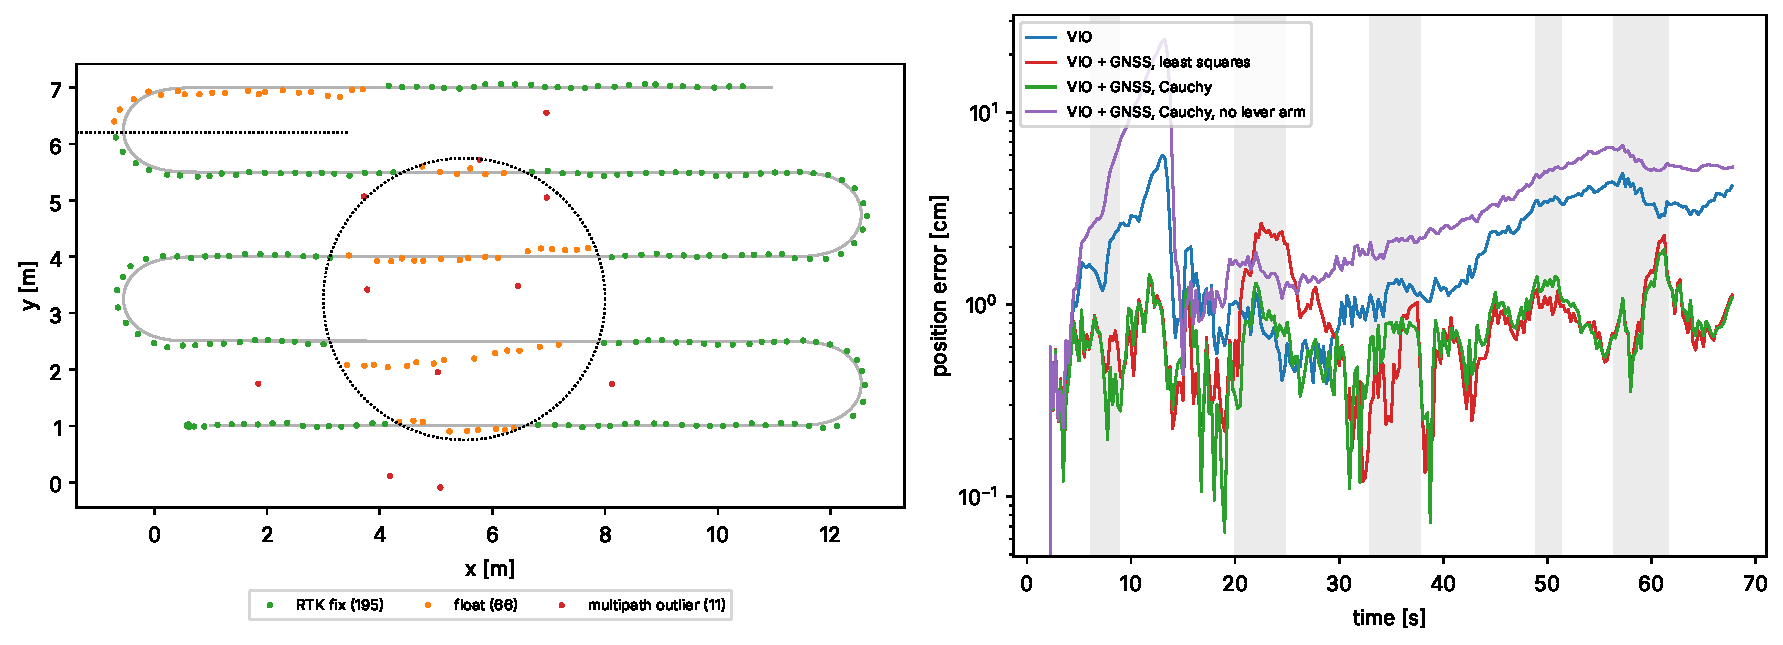
\includegraphics[width=\linewidth]{figures/ch14_gnss.pdf}
\caption{Left: the RTK measurements of the drive: fixes in the open,
float solutions under the tree (dotted circle) and near the house
(dotted line), and multipath outliers. Right: position errors of the
VIO and of the VIO with GNSS factors (grey bands: degraded GNSS).}
\label{fig:gnss}
\end{figure}

Of the 272 epochs of the drive, 72\,\% are fixed, 24\,\% float and 11
are multipath outliers with a median error of 2.3\,m (\cref{fig:gnss}).
With the GNSS factors in the window:
\begin{itemize}[nosep]
\item least squares on the reported uncertainties: 1.0\,cm RMS, 2.6\,cm
  at worst;
\item a Cauchy kernel on the whitened residual ($k=2$): 0.8\,cm RMS,
  1.9\,cm at worst, the outliers being down-weighted;
\item with the wheels as well: 0.9\,cm RMS, 1.7\,cm at worst;
\item without the lever arm: 5.5\,cm RMS and 24\,cm in the turns;
\item the VIO alone: 2.5\,cm RMS, and growing.
\end{itemize}
The difference between least squares and the Cauchy kernel is small
here, because the VIO is strong and the window holds only 2\,s: an
outlier is outvoted by the visual and inertial factors. It would not be
small for a GNSS-only filter, or for a VIO weakened by a blackout under
the same tree.

Over a 68\,s drive, the VIO alone is already good. The point of the GNSS
is the long run: a mowing session lasts an hour and covers kilometres,
and the VIO's error grows with the distance, whereas the error with GNSS
stays at the level of the fixes wherever the sky is open. A VIO strong
enough to bridge the canopy zones is what makes the combination work.

\begin{mower}
For the mower, this is where localisation becomes a product.
\begin{itemize}[nosep]
\item Mount the antenna high, with a clear view of the sky, and measure
  its lever arm to the body origin to a centimetre.
\item Use a base station within a few kilometres (one on the house roof
  works, as does an NTRIP service).
\item Expect the fix to drop under trees and along hedges and walls; the
  zones are the same from one session to the next, so they can be mapped
  and the GNSS factor de-weighted there in advance.
\item Measure the tyre radii, or better, estimate a wheel scale factor
  online.
\item Never let a GNSS position alone decide a boundary near the house
  or a flower bed. A multipath outlier of a metre looks exactly like a
  good fix.
\end{itemize}
\end{mower}

\begin{practice}[\code{vslam/fusion.py}, \code{vslam/vio.py}
  (\code{unary}, \code{transform}), \code{examples/ch14\_fusion.py},
  \code{notebooks/ch14\_fusion.ipynb}]
\begin{center}
\begin{tabular}{@{}ll@{}}
\toprule
Code & Formula\\
\midrule
\code{fusion.diff\_drive}, \code{wheel\_speeds} & \cref{def:diffdrive}\\
\code{fusion.dead\_reckon\_2d} & \cref{prop:deadreck}\\
\code{fusion.WheelFactor} & \cref{prop:wheelfactor}\\
\code{fusion.geodetic\_to\_ecef}, \code{R\_enu\_ecef} & \cref{prop:enu}\\
\code{fusion.GnssFactor} & \cref{prop:gnssfactor}\\
\code{fusion.align\_4dof} & \cref{prop:align4}\\
\code{SlidingWindowVIO.transform} & \cref{thm:vionull}\\
\code{fusion.Encoders}, \code{RTKReceiver} & simulated sensors\\
\bottomrule
\end{tabular}
\end{center}
The tests check the geodetic conversions and the ENU frame, the dead
reckoning covariance against Monte Carlo, the Jacobians of the wheel
and GNSS factors against finite differences, the 4-DoF alignment, and
that moving the whole window by a rotation about the vertical leaves its
cost unchanged.
\end{practice}

\section*{Further reading and C++ pointers}
\addcontentsline{toc}{section}{Further reading and C++ pointers}

GNSS and its fusion with inertial sensors: P.~D.~Groves, \emph{Principles
of GNSS, Inertial, and Multisensor Integrated Navigation Systems}, and
P.~J.~G.~Teunissen and O.~Montenbruck (eds.), \emph{Springer Handbook of
Global Navigation Satellite Systems} (2017). Integer ambiguity
resolution: the LAMBDA method of P.~J.~G.~Teunissen (Journal of Geodesy
1995). Wheels with VIO: K.~J.~Wu et~al., ``VINS on wheels'' (ICRA 2017).
GNSS in VIO: the global fusion of VINS-Fusion (T.~Qin et~al.), and
GVINS (S.~Cao, X.~Lu and S.~Shen, IEEE T-RO 2022), which uses the raw
GNSS measurements. In C++ and open source: RTKLIB (T.~Takasu) for RTK
processing, the \code{robot\_localization} package of ROS for EKF fusion
of wheels, IMU and GNSS, and GTSAM's \code{GPSFactor}.

\FloatBarrier
\section*{Exercises}
\addcontentsline{toc}{section}{Exercises}

\begin{enumerate}[label=\textbf{14.\arabic*},ref=14.\arabic*]
\item\label{ex:14radius} Two wheels of nominal radius 0.2\,m on a 1\,m
  track differ by 1\,mm in radius. How far off is the heading after a
  1\,km mowing session, with the wheels alone?
\item\label{ex:14offset} The body origin is a distance $d$ ahead of the
  axle. What sideways velocity does it have in a turn of yaw rate
  $\omega$, and how must \eqref{eq:wheelres} be changed?
\item\label{ex:14line} With fixes at 4\,Hz, $\sigma=1.5$\,cm and a speed
  of 1\,m/s, how far must the mower drive in a straight line before its
  heading is known to $0.1^\circ$?
\item\label{ex:14lever} Explain why leaving out the horizontal part of the
  lever arm hurts most in the turns, and why its vertical part matters
  only through tilt.
\end{enumerate}

\subsection*{Solutions}

\textbf{14.1.} A 1\,mm difference on 0.2\,m is $\epsilon_r-\epsilon_l=
0.5\,\%$. By \eqref{eq:wheelyaw}, $\delta\psi=0.005\times1000/1=5$\,rad:
the heading is meaningless after a few hundred metres. Wheel odometry
needs another source of heading.

\textbf{14.2.} The origin moves with $\vect{v}_o=\vect{v}_{\mathrm{axle}}+
\bomega\times(d,0,0)\T$, whose sideways component is $\omega d$. The
constraint applies to the axle, $R\T\vect{v}-\bomega\times(d,0,0)\T$, with
$\bomega$ the bias-corrected gyroscope rate; equivalently, place the body
origin of the VIO at the axle, as our implementation does.

\textbf{14.3.} With $n=4L$ fixes (one every 25\,cm),
$\sigma_\psi=\sigma\sqrt{12}/(L\sqrt{4L})=\sigma\sqrt3/L^{3/2}$. Setting
it to $0.1^\circ=1.75\times10^{-3}$\,rad gives
$L^{3/2}=0.015\sqrt3/1.75\times10^{-3}=14.8$, so $L=6.0$\,m.

\textbf{14.4.} The antenna is at $\p+R\vect{t}_{\mathrm{ant}}$. If the
lever arm is omitted, the estimator explains the measurements with
$\p$ alone. The horizontal part of $R\vect{t}_{\mathrm{ant}}$ is constant
along a straight row, so it is absorbed as a constant offset of the
trajectory, which is wrong by 0.4\,m but consistently so. In a turn it
rotates with the heading, by 0.8\,m between two rows, and no constant
offset explains that; the trajectory is dragged through the turn. The
vertical part, $(0,0,1.4)$\,m, has a horizontal projection of
$1.4\sin(\text{tilt})$, which changes only when the mower pitches or
rolls.
